\documentclass{article}
\usepackage{graphicx} % Required for inserting images
\usepackage[svgnames]{xcolor}
\usepackage[paperwidth=1000mm, paperheight=1200mm, margin=3cm]{geometry}
\usepackage{anyfontsize}
\usepackage{tikz}
\usepackage{mathpazo}
\usepackage{multicol}
\usepackage{blindtext}
\usepackage{tikz-cd}
\usepackage{amsmath}
\usepackage{amsfonts}

\usepackage{tikz}
\usetikzlibrary{decorations.pathreplacing,calc,tikzmark}

\renewcommand{\section}[1]{
    \begin{tikzpicture}
            \draw node[fill=yellow!80, text width=0.9\linewidth,
                text centered, inner sep=30pt, rounded corners=5pt,
                draw=yellow!80]
                {
                        \centering
                        \textbf{#1}
                };
        \end{tikzpicture}
}

\columnsep=60pt
\columnseprule=2pt

\begin{document}
\pagestyle{empty}
    \begin{center}
        \fontsize{65}{75}
        \selectfont
        \begin{tikzpicture}
            \draw node[fill=yellow!80, text width=0.95\linewidth,
                text centered, inner sep=30pt, rounded corners=5pt,
                draw=yellow!80]
                {
                    \begin{minipage}{0.20\textwidth}
                        \centering
                        
\includegraphics[width=0.7\textwidth]{logo_uniandes}\\

                        \bigskip
                        \bigskip
                        \bigskip
                        \bigskip
                        \bigskip
                        \bigskip

                        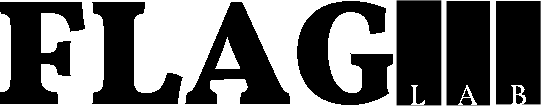
\includegraphics[width=0.7\textwidth]{Flag-logo.png}
                        
                        %
                    \end{minipage}%
                    \begin{minipage}{0.55\textwidth}
                        \centering
                        Quantum-safe lattice-based abstractions in functional programs\\[1cm]
                        \fontsize{50}{60}
                        \selectfont
                        \textbf{Daniel Barrero$^*$} \hspace{0.5cm} \textbf{Valérie Gauthier} \hspace{0.5cm} \textbf{Nicolás Cardozo}\\
                        \fontsize{40}{50}
                        \selectfont
                        Systems and Computing Engineering  - Universidad de los Andes\\
                        $^*$\texttt{dr.barrero2562@uniandes.edu.co}
                    \end{minipage}%
                    \begin{minipage}{0.25\textwidth}
                    \centering
                        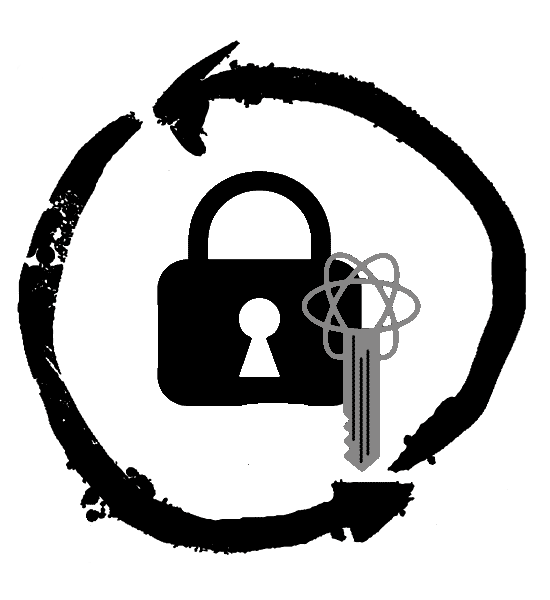
\includegraphics[width=0.25\textwidth]{crypto_0.png}

                        \bigskip
                        \bigskip
                        
\includegraphics[width=0.6\textwidth]{pil-logo.png}
                        %
\includegraphics[width=0.5\textwidth]{logo_uniandes.jpg}
                    \end{minipage}
                    
                };
        \end{tikzpicture}
    \end{center}
    \vspace{2cm}
    \begin{multicols*}{3}
        \fontsize{49}{59}
        \selectfont
        \section{Quantum-safe cryptography}\\
        
        Shor's quantum algorithm, published in 1994, demonstrated that factorization-based cryptography is no longer safe in the face of large-scale quantum computers.
        
        \[
    S_{i,j} =
        \begin{array}{ccccccc}
           \          & \      & |00\rangle & |01\rangle & |10\rangle & |11\rangle & \ \\
           |00\rangle & \vline & 1          & 0          & 0          & 0          & \vline\\
           |01\rangle & \vline & 0          & 1          & 0          & 0          & \vline\\
           |10\rangle & \vline & 0          & 0          & 1          & 0          & \vline\\
           |11\rangle & \vline & 0          & 0          & 0          & e^{i\theta_{k-j}}          & \vline
        \end{array}
\]


    %This begs the question of quantum-safe encryption protocols, for which \emph{the more, the better} rule applies.

    %For instance, the SIDH(KE) protocol was broken in 2022 by an efficient classical algorithm. ----> Have this to mention verbally, as I present the poster.


    % NIST standardization process, and its motivations.

    %In 2015, the NSA announced its transition to quantum-resistant algorithms, in recognition of threats such as (1) \emph{Harvesting attacks:} store today's keys and cyphertexts to break later, (2) \emph{Forging signatures for old keys}, (3) \emph{Implementing new cryptography at scale takes a long time}.
    
    In recognition of threats such as (1) \emph{Harvesting attacks:} store today's keys and cyphertexts to break later, (2) \emph{Forging signatures for old keys}, (3) \emph{Implementing new cryptography at scale takes a long time}.
    

    There are 4 main quantum-safe algorithms:

\noindent    
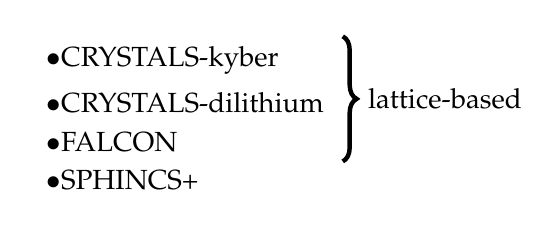
\begin{tikzpicture}
    \matrix (m) [matrix of nodes,column 1/.style={anchor=west}]
    {
    $\bullet$CRYSTALS-kyber \\
    $\bullet$CRYSTALS-dilithium \\
    $\bullet$FALCON \\
    $\bullet$SPHINCS+ \\
    };

    \draw [decoration={brace,amplitude=0.5em},decorate,ultra thick,black]
        (m-1-1.north -| m.east) --  node[right=0.5em]{lattice-based} (m-3-1.south -| m.east); 
\end{tikzpicture}
    
%    \begin{itemize}
%        \item CRYSTALS-kyber${}^*$
%        \item CRYSTALS-dilithium${}^*$
%        \item FALCON${}^*$
%        \item SPHINCS+
%    \end{itemize}

 
    \section{Lattice-based cryptography}\\
    
    Lattices offer the possibility of grounding cryptography on simple operations as matrix multiplication and vector addition, where a lattice is a periodic grid in space (of any dimension), defined as the $\mathbb{Z}$-span of a basis for $\mathbb{R}^n$:
    
    \fontsize{45}{45}
    \selectfont
    \[
        L(B) = \{a_1\mathbf{b_1} +...+ a_n\mathbf{b_n} | a_i \in \mathbb{Z}, \mathbf{b_i} \in B\}.
    \]

    \begin{center}
        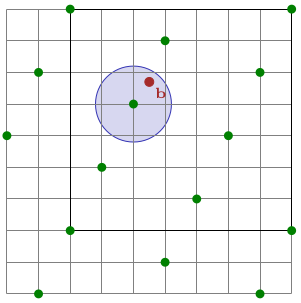
\includegraphics[width=0.22\textwidth]{lwe.png}
    \end{center}
    
    \fontsize{49}{58}
    \selectfont

    Computationally hard problems arise when the dimension of the lattice becomes large. In the relation
    
    % the most essential example being the \emph{shortest vector problem} (SVP, SVP${}_\gamma$).
    
    % In the related \emph{learning with errors} (LWE) problem, a public key cryptosystem is given by the relation

    \[
        \mathbf{b}^t = \mathbf{s}^t \mathbf{A} + \mathbf{e}^t,
    \]

    the public key is the random matrix $\mathbf{A}$ and the secret key is the vector $\mathbf{s}$. Recovering such key from the cyphertext $\mathbf{b}$ is as hard as solving the \emph{shortest vector problem} (SVP, SVP${}_\gamma$), which is known to be NP-hard.\\

    \section{Current shortcomings}
 
 \bigskip 
 
PQC algorithm are known to have a :
    \begin{itemize}
        \item \textbf{{\color{red} 2.3x run-time}} overhead
        \item \textbf{{\color{red} 3.1x energy}} consumption increase
        \item \textbf{{\color{red} 70x more data}} overhead
    \end{itemize}

    These complications are due to internal hashing and \emph{discrete Fourier transforms} (DFTs), which occur iteratively in the encryption process.\\

To \textbf{{\color{ForestGreen} improve performance}} and \textbf{{\color{ForestGreen} alleviate the complexity}} of building quantum-safe algorithms we proposed to use \textbf{advanced algebra concepts} from a \textbf{programming language perspective}.

    \bigskip
    \section{Operad-based cryptography}
   
    \bigskip

     The crypto-standard rely on property-preserving transformations (i.e., homomorphisms) to simplify computational complexity 
     
     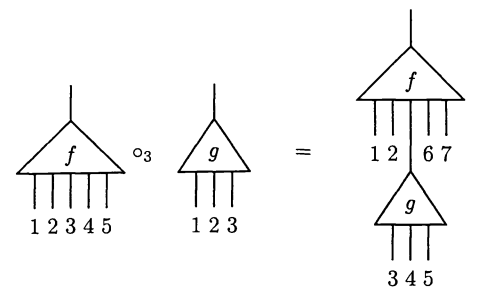
\includegraphics[width=0.29\textwidth]{fig1Intromss02.png}
     
     Our hypothesis is that sequences of operations can be further simplified using the theory of \emph{operads}, whose objects represent \emph{operation composition}.
    
    \bigskip
    \bigskip
    \bigskip
    \bigskip
    \bigskip
    
    \section{A declarative language for quantum-safe cryptography} 

\bigskip
\bigskip
\bigskip
\bigskip
\bigskip

    \begin{itemize}
        \item Cryptography protocols are implemented in languages such as C, which lack the expressiveness for algebraic operations or composition. This adds computational overhead and hides the intrinsic complexity of the scheme.
        \item Functional languages (e.g., Haskell) allow programmers to define category-theoretic abstractions appropriate for a mathematically \textbf{clear and natural operation composition}. 
        \bigskip
        \item[] \begin{center} 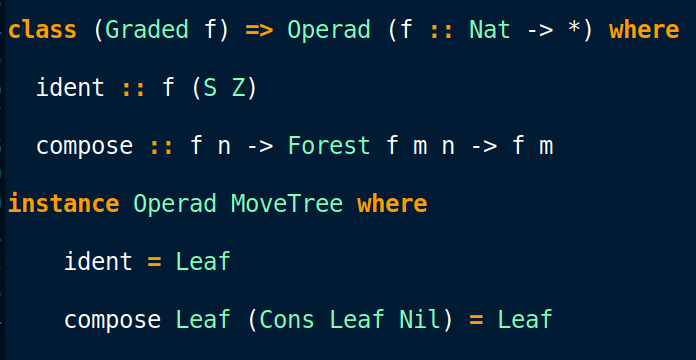
\includegraphics[width=0.3\textwidth]{toyOpds.png} \end{center}
        \bigskip
        \item In this project, we propose the \texttt{\textbf{SILVER}} language. %Safely Implemented, Lattice-based Verifiable Encryption Resource.
    Following the correspondence between mathematical definitions and type/typeclass declarations in our purely functional language, together with the use of a sound type specification system for program execution to create a \textbf{simple, safe, expressive, performant}, and \textbf{maintainable} programming language for quantum-safe cryptography.
    \end{itemize}
    
    
    \end{multicols*}
        
\end{document}
